\documentclass{standalone}

\usepackage{tikz}

\usetikzlibrary{quantikz2}

\begin{document}

    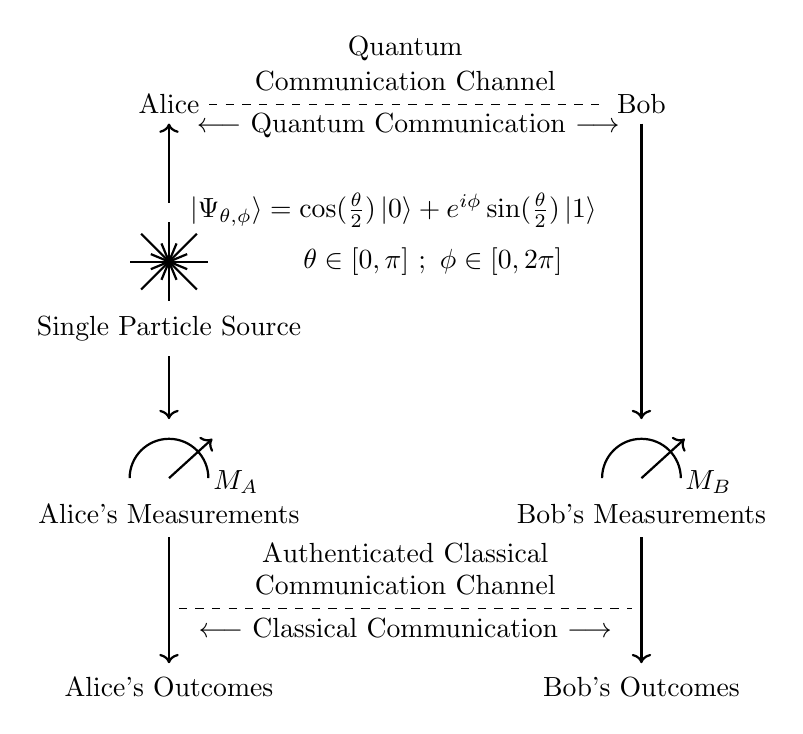
\begin{tikzpicture}
        \node (alice) at (-3, 0) {Alice};
        \node (bob) at (3, 0) {Bob};
        
        \node (alice-terminal) at (-3, -6.4) {};
        \node (bob-terminal) at (3, -6.4) {};

        % Quantum communication
        \draw[dashed] (alice) -- (bob) node[midway, below] {$\longleftarrow$ Quantum Communication $\longrightarrow$};
        \node at (0, 0.7) {Quantum};
        \node at (0, 0.3) {Communication Channel};
    
        % Alice's quantum device
        \draw[thick,->] (-3, -1.25) -- (alice) node[below] {};
        \draw[thick,->] (-3, -3.2) -- ++(0, -0.8) node[below] {};
    
        % Bob's quantum device
        \draw[thick,->] (bob) -- ++(0, -4) node[below] {};
        
        % Define the center of the spark
        \coordinate (center) at (-3,-2);
        % Define the points of the spark
        \foreach \angle in {0, 45, 90, 135, 180, 225, 270, 315} {
            \draw[thick, black] (center) -- ++(\angle:0.5cm);
        }
        % Define inner lines to create a spark look
        \foreach \angle in {22.5, 67.5, 112.5, 157.5, 202.5, 247.5, 292.5, 337.5} {
            \draw[thick, black] (center) -- ++(\angle:0.25cm);
        }
        
        % Labels for the single particle source
        \node at (-3, -2.85) {Single Particle Source};
    
        % Classical communication
        \draw[dashed] (alice-terminal) -- (bob-terminal) node[midway, below] {$\longleftarrow$ Classical Communication $\longrightarrow$};
        \node at (0, -5.7) {Authenticated Classical};
        \node at (0, -6.1) {Communication Channel};

        % Draw the Alice's measurement needle
        \draw[thick] (-2.5,-4.75) arc (0:180:0.5cm);
        \draw[thick, ->] (-3,-4.75) -- (-2.45,-4.25);
        \node at (-2.15, -4.8) {$M_A$};

        % Draw the Bob's measurement needle
        \draw[thick] (3.5,-4.75) arc (0:180:0.5cm);
        \draw[thick, ->] (3,-4.75) -- (3.55,-4.25);
        \node at (3.85, -4.8) {$M_B$};
        
        % Labels for the measurements
        \node at (-3, -5.2) {Alice's Measurements};
        \draw[thick, ->] (-3,-5.5) -- (-3,-7.1);
        \node at (3, -5.2) {Bob's Measurements};
        \draw[thick, ->] (3,-5.5) -- (3,-7.1);
    
        % Labels for the outcomes
        \node at (-3, -7.4) {Alice's Outcomes};
        \node at (3, -7.4) {Bob's Outcomes};
    
        % Labels for the entanglement states
        \node at (-0.15, -1.35) {$\ket{\Psi_{\theta,\phi}} = \cos(\frac{\theta}{2}) \ket{0} + {e}^{i \phi} \sin(\frac{\theta}{2}) \ket{1}$};
        \node at (0.35, -2) {$\theta \in [0, \pi]\ ;\ \phi \in [0, 2\pi]$};
    \end{tikzpicture}

\end{document}